The density ratio is defined \citep{ulrich_1972}
%Do this in terms of N^2
\begin{equation}
    R_\rho = \frac{\nabla_T - \nabla_{\rm{ad}}}{{\nabla_\mu}},
\end{equation}
where $\nabla_T$ is the logarithmic temperature gradient, $\nabla_{\rm{ad}}$ is its adiabatic value, and $\nabla_\mu$ is the Ledoux composition gradient term.
Throughout this section, we report mixing efficiency assuming that thermohaline mixing can be modeled as a diffusivity with diffusion coefficient $D_{\rm{th}}$; this quantity can be converted to the Nusselt number $\mathrm{Nu}_{\rm{th}}$ in the fluid dynamics literature using the formula $D_{\rm{th}} = (\mathrm{Nu}_{\rm{th}} - 1)\kappa_\mu$, where $\kappa_\mu$ is the compositional diffusivity. 

The default thermohaline mixing model in the MESA software instrument \citep{mesa2} was originally derived by \citet{ulrich_1972, kippenhahn_etal_1980}.
Thermohaline mixing is treated as a diffusion process, with a diffusion coefficient
\begin{equation}
    D_{\rm{th}} = \alpha_{\rm{th}} \frac{3 K}{2\rho C_P}R_{\rho}^{-1}.
    \label{eqn:kipp_model}
\end{equation}
\textcolor{blue}{[Might be worth also writing it in terms of $\tau$, see the last paragraph in section 3.1 of Traxler ApJ 2011]} Here, $\alpha_{\rm{th}}$ is a dimensionless efficiency parameter, $K$ is the radiative conductivity, $\rho$ is the density, and $C_P$ is the specific heat at constant pressure. 

\citet{traxler_etal_2011} derive a mixing law by fitting a function to a large set of simulations.
They define the reduce density ratio, $r \equiv (R_0 - 1)/(\tau^{-1} - 1)$, where $\tau = \kappa_\mu/\kappa_T$ is the ratio of compositional to thermal diffusivity.
They find that
\begin{equation}
   D_{\rm{th}} = \kappa_{\mu}\sqrt{\frac{\mathrm{Pr}}{\tau}}\left(a e^{-br}[1 - r]^c\right),
    \label{eqn:trax_model}
\end{equation}
where $\mathrm{Pr} = \nu / \kappa_T$ with $\nu$ the viscosity, and they find $a = 101 \pm 1$, $b = 3.6 \pm 0.3$, and $c = 1.1 \pm 0.1$.



\citet{brown_etal_2013} note that the model in Eqn.~\ref{eqn:trax_model} performs well at high $R_\rho$, but underestimates mixing at low $R_\rho$, particularly in the stellar regime of low Pr and $\tau$.
They develop a semi-analytical model for thermohaline mixing,
\begin{equation}
    D_{\rm{th}} = \kappa_{\mu}C^2\frac{\lambda^2}{\tau l^2(\lambda + \tau l^2)},
    \label{eqn:brown_model}
\end{equation}
where $\lambda$ is the growth rate of the fastest growing linearly unstable mode, $l$ is its horizontal wavenumber, and $C \approx 7$ is a universal constant which they fit to simulation data.
Obtaining $\lambda$ and $l$ requires solving a cubic and quadratic equation (their Eqns.~19 and 20).

These new implementations are used in \citep{bauer_bildsten_2019} and other works.

(cite) paper is the paper that implements these new models in MESA and it's been there since r(put revision here)


\citet{harrington} build on the model of \citet{brown_etal_2013} by including magnetic fields and find that magnetism can increase mixing efficiency.
They utilize the same Eqn.~\ref{eqn:brown_model} but define the velocity of the instability $\hat{w}_f^2 = \lambda^2/l^2$ for clarity. 
Their Eqn.~32 provides an expression for $\hat{w}_f^2$ which depends on the magnitude of the magnitude field $B_0^2$.
This expression has two asymptotic limits, in which $\hat{w}_f^2 \propto B_0^2$ when $B_0$ is large, and which reduces exactly to the model of \citet{brown_etal_2013} when $B_0$ is small.
(this is a new model that is not yet implemented in MESA).


There has been other work regarding multi-D models of thermohaline mixing \citep{denissenkov_2010, denissenkov_merryfield_2011}, but 2D thermohaline behaves very differently from 3D thermohaline \citep{garaud_brummell_2015}, and so we do not consider that set of data in this work.

\citet{lattanzio_etal_2015} tested one or multiple of these models in a bunch of different codes on the RGB and found X.
In this paper, we will determine if observations are capable of probing the differences between these different models are not.

\begin{figure}
    \centering
    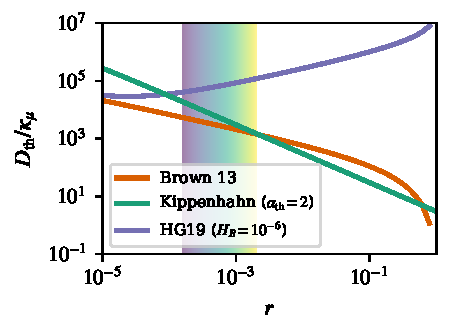
\includegraphics[width=\columnwidth]{Nu_models_comparison.pdf}
    \caption{\textcolor{red}{[Todo: Add MHD models.]}}
    \label{fig:parameterization_compare}
\end{figure}

\textbf{Adrian}: Start making this plot
Do you need to discuss here? or cite previous work? include plot of Nu vs R0 with the different model/theory predictions, mark simulations, like you did for bring a plot [AF: assuming I finally wrap up my in-prep paper with Pascale, we can just cite that paper and throw in those Nu vs R0 plots]
